\section{Atividade 4}

\subsection{Descrição do Modelo e Simulação}
Nesta atividade, analisamos um sistema de controle típico. Utilizamos um controlador proporcional cujo ganho \( K \) é determinado pela relação \( \frac{m}{3} \), onde \( m \) é a massa do sistema. A função de transferência da planta (Gp) é derivada da equação dinâmica da massa, amortecimento e constante da mola, especificada na Atividade 3. O sensor é modelado por um sistema de primeira ordem, com ganho unitário \( K_s = 1 \) e constante de tempo \( T_s = \frac{m}{6} \).

\subsection{Construção do Diagrama de Blocos}
Abaixo, apresentamos o diagrama de blocos para o sistema de controle, ilustrando a interação entre o controlador, a planta e o sensor.

\begin{figure}[H]
    \centering
    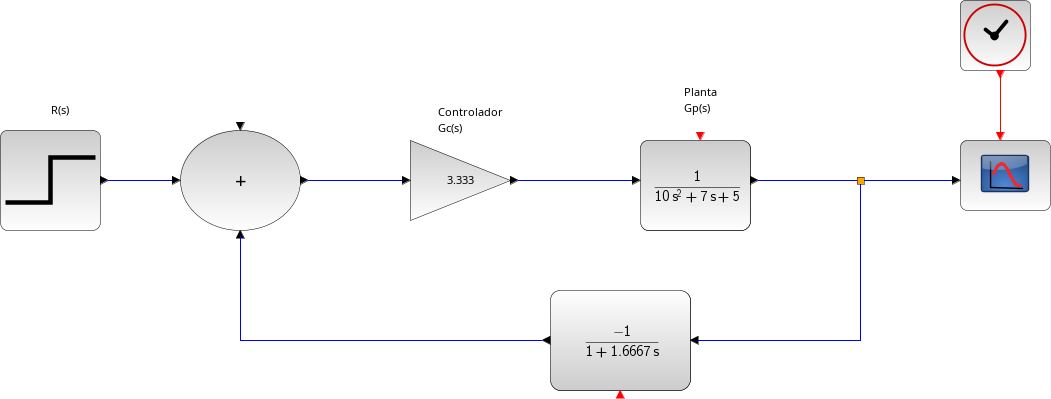
\includegraphics[width=0.7\textwidth]{4-atividade/assets/diagrama.png}
    \caption{Diagrama de blocos do sistema de controle}
    \label{fig:diagrama_blocos}
\end{figure}

As funções de transferência são especificadas como segue:
\begin{itemize}
    \item Controlador: \( G_c(s) = \frac{m}{3} \) com \( m = 10 \), então \( G_c(s) = \frac{10}{3} \)
    \item Planta: \( G_p(s) = \frac{1}{m s^2 + C s + K} = \frac{1}{10 s^2 + 7 s + 5} \)
    \item Sensor: \( H(s) = \frac{1}{1 + \frac{m}{6} s} = \frac{1}{1 + 1.6667 s} \)
\end{itemize}

\subsection{Função de Transferência em Malha Fechada}
Calculamos a função de transferência em malha fechada \( C(s)/R(s) \) pela fórmula:
\[
    G_{closed}(s) = \frac{G_c(s) \cdot G_p(s)}{1 + G_c(s) \cdot G_p(s) \cdot H(s)}
\]
Substituímos as funções de transferência obtidas:
\[
    G_{closed}(s) = \frac{\frac{10}{3} \cdot \frac{1}{10 s^2 + 7 s + 5}}{1 + \frac{10}{3} \cdot \frac{1}{10 s^2 + 7 s + 5} \cdot \frac{1}{1 + 1.6667 s}}
\]
Simplificamos a expressão para chegar à forma final da função de transferência em malha fechada:
\[
    G_{closed}(s) = \frac{0.3333333s + 0.2}{s^3 + 1.3s^2 + 0.92s + 0.5}
\]

\subsection{Análise de Estabilidade pelo Critério de Routh-Hurwitz}
Utilizamos o critério de Routh-Hurwitz para avaliar a estabilidade do sistema, baseando-nos nos coeficientes do denominador da função de transferência em malha fechada.

\subsubsection{Resultados da Análise de Estabilidade}
A matriz de Routh-Hurwitz, obtida a partir dos coeficientes do polinômio do denominador, é apresentada a seguir:
\[
    RH\_matrix = \begin{bmatrix}
        0.5  & ... \\
        0.92 & ... \\
        1.3  & ... \\
        1    & ... \\
    \end{bmatrix}
\]
O sistema é considerado estável, pois todos os elementos da primeira coluna são positivos.

\subsection{Análise de Estabilidade para Diferentes Valores de \( K \)}
Investigamos a estabilidade do sistema para diferentes valores do ganho do controlador \( K_p \), variando de 1 a 10. As análises mostram que o sistema mantém a estabilidade em todo o intervalo testado.

\subsubsection{Resultados da Resposta ao Degrau}
Abaixo, apresentamos o gráfico da resposta ao degrau para os diferentes valores de \( K_p \):

\begin{figure}[H]
    \centering
    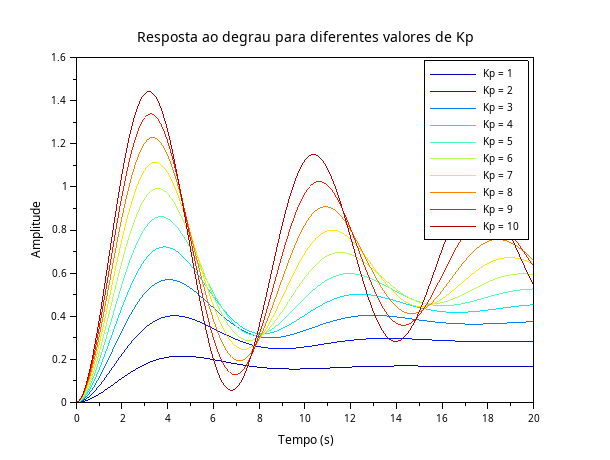
\includegraphics[width=0.7\textwidth]{4-atividade/assets/impulsos-diferentes-kp.png}
    \caption{Resposta ao degrau para diferentes valores de \( K_p \)}
    \label{fig:resposta-degrau-kp}
\end{figure}

\subsection{Conclusões}
As análises mostram que o sistema massa-mola-amortecedor controlado proporcionalmente é estável para os valores de \( K_p \) entre 1 e 10. Observa-se que o comportamento da resposta ao degrau varia significativamente com o ganho do controlador, destacando a necessidade de ajuste adequado para alcançar a resposta desejada do sistema.
